\chapter{Further developments}

\section{Distributed testing}

In order to scale, the framework should be able distribute tests to a network of Daemon nodes (target distributions). One way of doing so is by using "local networks". It is defined as a collection on Daemons and the Engine instance connected to them. The Engine should make the set of Daemons available to any Controller that joins its network. Through the UI a tester can then select not only the tests to be run, but also the targets. The initial implementation could simply broadcast the set of tests to all selected Daemons, but with a good enough UI, test selection could also be Daemon specific. The results could be provided as a bundle by the Engine, or sent directly to the Controller which will wait for them.

\begin{figure}[h!]
  \centering
	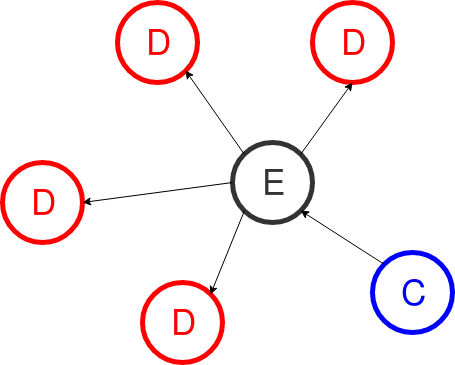
\includegraphics[width=0.4\textwidth]{images/local.png}
    \caption{Example of a local network}
\end{figure}

In order to make the system scalable not only with the number of target devices, but also with the number of parallel instances of Daemons running on the same distribution, a dependency tracking and checking system between tests must be implemented. 

\subsection{Access control and network labels}

By using local networks defined as a set of Daemons and an Engine, an access control system could de implemented that uses Controller identification and defines what access rights should be offered.

Additional functionality can be provided by labeling. A local network could be limited to a specific task - run tests for a single requirement on multiple types of targets or run tests from the same provider even if they test different requirements. 

\section{Test profiles}

When writing a test suite, a vendor or community will have subjective views about what validation means, or when a requirement is truly validated. This can lead to different test suites for the same specification. These different branches could be viewed as "profiles" of the same specification and would benefit all if brought under a publicly available service. Vendors could start by building on already existing suites while the rest of community will be able to judge how well the specification is tested. The process will be accelerated and will become very transparent. From a technical point of view, it would mean that the test suites available on the targets and used by the Daemons will need a versioning system and identification.

% \begin{figure}[h!]
%   \centering
% 	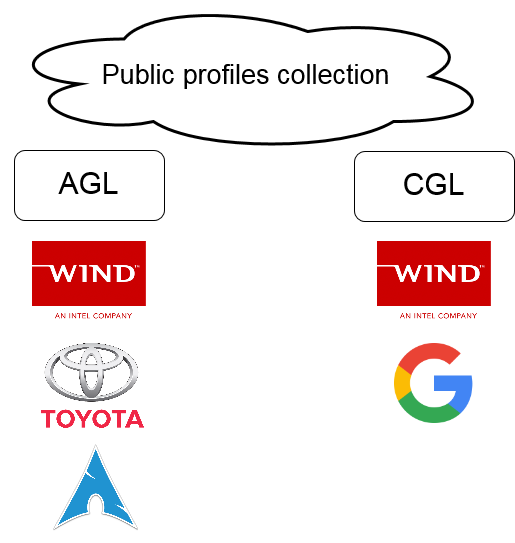
\includegraphics[width=0.5\textwidth]{images/profiles.png}
%     \caption{A public profile repository}
% \end{figure}
